
In recent years, the popularity of the Internet has soared. 
One of the more popular uses of the Internet is instant messaging. 
In this chapter, a distributed instant messaging system 
is presented to illustrate the use of the C ORB Interface 
System with the Standard ML of New Jersey compiler. 

\section*{\underline{SYRUP: Simple Yet Reliable Utility for Product Planning}}
\addcontentsline{toc}{section}{SYRUP: Simple Yet Reliable Utility for Product Planning}

Suppose a group of young entrepreneurs would like to start a 
corporation.  Also suppose that these young entrepreneurs live very 
far apart.  Since they live so far apart, meeting in person is simply 
not practical.  They also don't have a lot of money to waste on long 
distance telephone calls.  Therefore, they need some other means by which 
to communicate.  Since, Internet instant messaging provides a cost-effective 
solution to their dilemma, they elect to create their own instant messaging 
system that they can use to plan their corporate strategy and product line.   
In addition to the need for instant messaging capability, they would also 
like this application to provide the ability to post ideas on a message 
board that is accessible via a web browser.   

This scenario involving the young entrepreneurs provides an excellent 
opportunity to create a CORBA based application.  Since each entrepreneur 
could be using a different computing platform, we need to make sure 
that we can create components that can inter-operate with ease.  CORBA 
provides us with that ability.  Since there are many programming languages 
that can take advantage of CORBA capabilities, we need to select the 
language or languages that provide the most capability in the domain of 
our problem.  Because the distribution of the instant messaging application
will also be a concern, it would be nice if we could take advantage of 
JAVA's Applet facilities.  This way, the only software needed on each 
entrepreneur's computer is a web browser.  JAVA will also provide 
our client application with elegant graphical user interface features. 
Now that we have decided to implement our client application in JAVA, 
we must decide which programming language to use in the implementation 
of our instant messaging server.  This component will be responsible 
for maintaining a list of users that are currently using the system 
and are accepting instant messages.  It will also be responsible for 
passing instant messages from one user to another and writing messages 
on the message board.    Since ML offers a built-in list data type and 
a rich set of list manipulation features, the instant messaging server 
is an excellent opportunity to use the CORBin System to implement a 
CORBA object in ML.  
A diagram of the S$.$Y$.$R$.$U$.$P$.$ System is illustrated in figure 
\ref{SyrupComponentDiagram}.  
\begin{figure}
\begin{center}
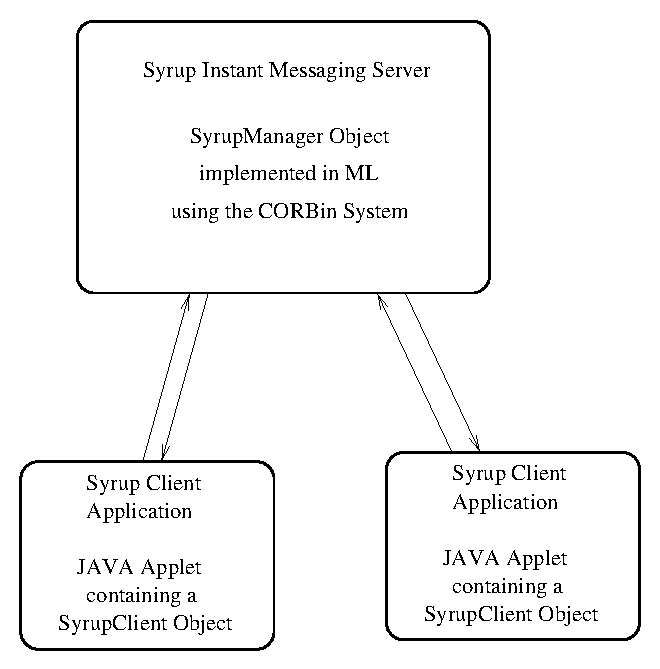
\psfig{file=Figures/SyrupComponentDiagram.eps}
\leavevmode
\caption{\em{Diagram of the S$.$Y$.$R$.$U$.$P$.$ System}.}
\figline
         \label{SyrupComponentDiagram}
\end{center}
\end{figure}

Notice that the instant messaging server must have the ability to 
communicate with each client application in addition to serving 
client application requests.   This also provides an excellent 
opportunity use a CORBA design pattern called {\em{callback}}. 
Using the CORBA callback pattern, the client application will pass 
a reference to a CORBA object to another CORBA object.  The receiving 
object can then retain the object reference to later invoke 
operations on it. Therefore, in addition to communicating with a remote CORBA
object, our client application will also contain a CORBA object that the 
instant messaging server can invoke operations on.  
Since we are using the callback pattern, the CORBA object we implement in ML
will not only illustrate how to use the CORBin system can be used to 
implement CORBA objects, it will also allow us to illustrate how ML 
can communicate with remote CORBA objects.

\section*{\underline{The Design}}
\addcontentsline{toc}{section}{The Design}

Before we can create an IDL specification for our application, we must 
determine what functionality is needed by our CORBA objects.  Clearly, 
we need some means by which users can register and unregister themselves
as S$.$Y$.$R$.$U$.$P$.$ users.  Therefore, our SyrupManager object should 
have the ability to allow users to {\em{Login}} and {\em{Logout}}.  
Also, it should provide functionality to allow users to {\em{send messages}} 
to one another. As a final requirement, the SyrupManager object should allow 
users to {\em{post messages}} to an electronic bulletin board.  These 
ideas are illustrated using the Unified Modeling Language (UML) in figure 
\ref{SyrupManagerUseCases}. 
\begin{figure}
\begin{center}
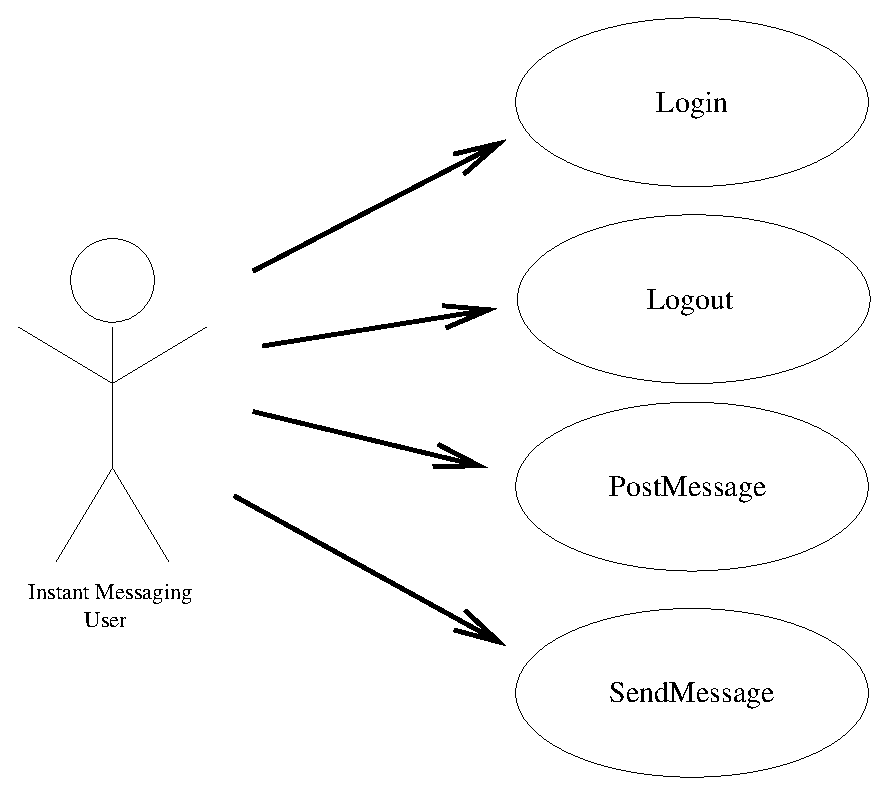
\psfig{file=Figures/SyrupManagerUseCases.eps}
\leavevmode
\caption{\em{UML Use Cases for the SyrupManager Object}.}
\figline
         \label{SyrupManagerUseCases}
\end{center}
\end{figure}

The SyrupManager object also requires some functionality to be included 
in the SyrupClient object.  First, The SyrupManager needs 
to be able to add and remove users from a list of users that are currently 
available to receive instant messages.  In addition to these requirements, 
the SyrupClient object must also include functionality to allow for the 
delivery of instant messages. These ideas are also illustrated using UML in 
figure \ref{SyrupClientUseCases}.
\begin{figure}
\begin{center}
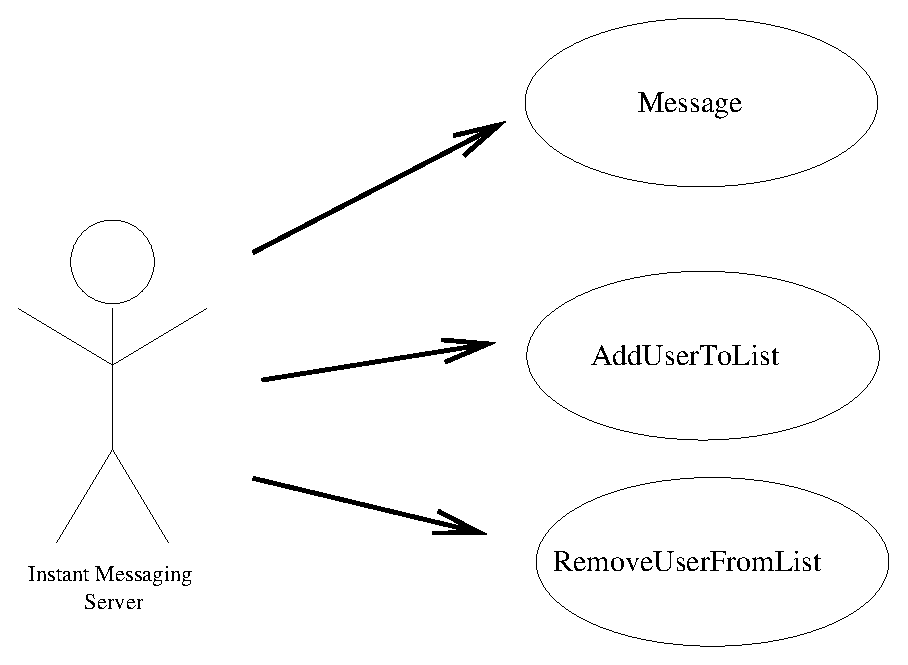
\psfig{file=Figures/SyrupClientUseCases.eps}
\leavevmode
\caption{\em{UML Use Cases for the SyrupClient Object}.}
\figline
         \label{SyrupClientUseCases}
\end{center}
\end{figure}

Now that we know the required functionality of each object, we can construct 
UML class diagrams that illustrate the necessary parameters and their types for 
each operation.  The operations that belong to the SyrupManager object are 
shown in figure \ref{SyrupManagerClassDiagram} and the operations that belong 
to the SyrupClient object are shown in figure \ref{SyrupClientClassDiagram}.   
Notice that the {\em{Login}} operation of the SyrupManager object requires two 
parameters: a string representing a user name and a reference to a SyrupClient 
object.  This allows the SyrupManager object to send updates back to that 
client application.
\begin{figure}
\begin{center}
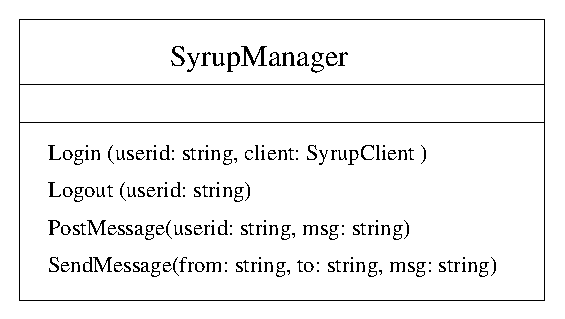
\psfig{file=Figures/SyrupManagerClassDiagram.eps}
\leavevmode
\caption{\em{UML Class Diagram for the SyrupManager Object}.}
\figline
         \label{SyrupManagerClassDiagram}
\end{center}
\end{figure}
\begin{figure}
\begin{center}
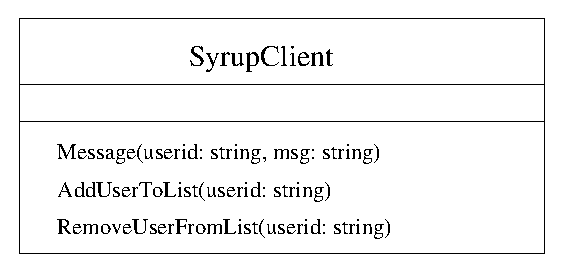
\psfig{file=Figures/SyrupClientClassDiagram.eps}
\leavevmode
\caption{\em{UML Class Diagram for the SyrupClient Object}.}
\figline
         \label{SyrupClientClassDiagram}
\end{center}
\end{figure}


\section*{\underline{Interface Definition}} 
\addcontentsline{toc}{section}{Interface Definition}

Recall that before we can implement a CORBA object in a programming 
language, we must define the interface by which other CORBA objects 
may utilize our object's functionality. The IDL specification for 
our instant messaging application is listed in figure \ref{syrupIDL}.
Notice the use of the IDL keyword {\em{oneway}}.
Here, we use the {\em{oneway}} keyword when we do not want to wait on 
the operation to return before we can continue processing.  This 
{\em{oneway}} feature of CORBA is implemented in various degrees 
of robustness by ORB vendors. It should be noted that if you must 
know that the parameters were correctly received by the remote 
object then the {\em{oneway}} attribute should probably not be used. 
Upon completion of the IDL specification, corbin-idl is used to 
generate IDL stubs, IDL skeletons, and rebuild the SML/NJ runtime 
system. 
\begin{figure*}[t]
\singlespace
\begin{verbatim}

  module Syrup {

        interface SyrupClient  {

                oneway void Message(in string userid, 
                                    in string msg);	
                oneway void AddUserToList(in string userid); 
                oneway void RemoveUserFromList(in string userid); 
        };

        interface SyrupManager {
	
                void Login  (in string userid, 
                             in SyrupClient client); 
                void Logout (in string userid);		
                oneway void PostMessage (in string userid, 
                                         in string msg);
                oneway void SendMessage (in string from, 
                                         in string to,
                                         in string msg);

        };

  };

\end{verbatim}
\doublespace
\caption {{\em IDL specification for the S$.$Y$.$R$.$U$.$P$.$ Instant Messaging Application}.}
\figline
        \label{syrupIDL}
\end{figure*}



\section*{\underline{IDL Skeleton Implementation}}
\addcontentsline{toc}{section}{IDL Skeleton Implementation}

Once we have compiled the IDL specification for our application, we must 
implement the CORBA objects in a programming language.  In this case, we
must implement the operations of the SyrupManager object in ML so that 
a client application can use it to communicate with other Syrup users. 
The ML code used to implement the SyrupManager operations is listed in 
figure \ref{SyrupManagerInML}. 
\begin{figure*}[t]
\singlespace
\begin{verbatim}


fun Login [Cstring id, Caddr obj] = 
          (SyrupManager.add_user_to_list(id,obj);
           Cint(0w1) )
fun Logout [Cstring id] = 
          (SyrupManager.remove_user_from_list(id);
           Cint(0w1) )
fun PostMessage [Cstring id, Cstring msg] = 
          (SyrupManager.write_message(id, msg);
           Cint(0w1) )

fun SendMessage [Cstring from, Cstring to, Cstring msg] = 
          (SyrupManager.send_message(from,to, msg);
           Cint(0w1) )

val _ = CORBin_Syrup_SyrupManager_Login_SetMLFn(Login);
val _ = CORBin_Syrup_SyrupManager_Logout_SetMLFn(Logout);
val _ = CORBin_Syrup_SyrupManager_PostMessage_SetMLFn(PostMessage);
val _ = CORBin_Syrup_SyrupManager_SendMessage_SetMLFn(SendMessage);

\end{verbatim}
\doublespace
\caption {{\em SyrupManager Implementation in ML}.}
\figline
        \label{SyrupManagerInML}
\end{figure*}
Notice that each function takes a list as a parameter.  This list is 
composed of data types defined in a SML/NJ library that accompanies the 
SML/NJ C interface.  These data types represent their counterparts in the 
C programming language.  Also notice that although these functions were defined 
to have no return value in the IDL specification, the CORBin System requires 
that void functions return an integer value.  In order to modularize 
our implementation of the SyrupManager object, a separate ML structure has 
been defined that contains various utility functions.  Excerpts from this 
structure are listed in figure \ref{SyrupManagerStructure}.  The full 
source code listing for the SyrupManager structure is presented in the 
appendix.   
\begin{figure*}[t]
\singlespace
\begin{verbatim}

val user_list: (string * caddr) list ref  = ref []

fun add_user_to_clients_gui(id: string, nil) =  ()
  | add_user_to_clients_gui(id: string, 
                          (uid: string, obj: caddr)::rest) =
    (if (id = uid) then
        add_user_to_clients_gui(id, rest)
     else
        (CORBin_Syrup_SyrupClient_AddUserToList(obj, id);
         add_user_to_clients_gui(id, rest)))

fun add_users_to_new_clients_gui(obj: caddr, nil) =  ()
  | add_users_to_new_clients_gui(obj: caddr,
                          (uid: string, uobj: caddr)::rest) =
    (CORBin_Syrup_SyrupClient_AddUserToList(obj, uid);
     add_users_to_new_clients_gui(obj, rest))


fun add_user_to_list (id: string, obj: caddr) =
    let val obj_copy = CORBin_Object_duplicate(obj)
    in
          user_list := (id,obj_copy)::(!user_list);
          add_user_to_clients_gui(id, !user_list);
          add_users_to_new_clients_gui(obj_copy, !user_list)
    end

\end{verbatim}
\doublespace
\caption {{\em Excerpts from an ML structure providing utility functions to our SyrupManager implementation}.}
\figline
        \label{SyrupManagerStructure}
\end{figure*}

In order to illustrate the process of implementing a CORBA object in ML using 
the CORBin System, we will now discuss the Login operation of the SyrupManager 
object in detail.  In figure \ref{SyrupManagerInML}, you will notice that the 
the Login operation calls a function, {\em{add\_user\_to\_list}}, that is 
defined in a structure called SyrupManager.
The code for this function is listed in figure \ref{SyrupManagerStructure}.   
Notice that {\em{add\_user\_to\_list}} first calls {\em{CORBin\_Object\_duplicate}} 
to increment the reference count for the object reference of the SyrupClient 
object we received from the client application.  This is done since ORBit 
object references maintain a reference count in order to determine if they are 
still in use.   Once this has been done, we add the string representing the 
user's screen name and the SyrupClient object reference to a list as a tuple.  
Now, we must notify other users that a new user has just logged in to the system. 
The reason this is of interest is because it illustrates how ML programmers can 
communicate with other CORBA objects with the CORBin System.  Notice that the 
first line of the {\em{add\_user\_to\_clients\_gui}} function is a call to the 
{\em{CORBin\_Syrup\_SyrupClient\_AddUser\-ToList}} function.  This should look somewhat
familiar as this function was generated by corbin-idl when the IDL specification
for the S$.$Y$.$R$.$U$.$P$.$ application was processed.  As with all CORBin related 
functions, this function name begins with CORBin.  The rest of the name is composed 
of {\em{module name}} (Syrup), {\em{interface name}} (SyrupClient), and 
then {\em{operation name}} (AddUserToList).  Each name is separated by the underscore
character.  The object reference for the remote object is always the first parameter
passed to an IDL stub function generated by corbin-idl. Any additional parameters 
are passed after the object reference in the order in which they are defined in the 
IDL specification.   This naming convention is used for all IDL stub functions 
generated by corbin-idl.  Now that the Login operation has been implemented in ML, 
we must register it with the CORBin System so that client applications may utilize it.
This is done by passing the name of the function that implements the operation to 
a function generated by corbin-idl.  This function saves a pointer to the ML function 
that implements the operation so that when requests arrive to execute the operation, 
this function pointer is used to execute the ML code necessary to complete the operation.   
In order to establish that the ML function {\em{Login}} implements the Login operation
of the SyrupManager object, we call the {\em{CORBin\_Syrup\_SyrupManager\_Login\_SetMLFn}}
function. The naming convention for these function registration routines is similar 
to the IDL stub functions except {\em{SetMLFn}} is appended to the end of the function 
name.  Before activating a CORBA object implemented using the CORBin System, 
the programmer should always register a function that implements each operation 
defined for the object. 

Once the ML programmer has implemented the operations of a CORBA object with 
ML functions and registered those functions, some additional work must be done 
before this object can be used by a client application.  The code needed to 
{\em{activate}} our SyrupManager implementation in ML is listed in figure 
\ref{MLObjectActivate}. This setup process should look familiar to experienced 
CORBA developers.  This process involves creating a SyrupManager object, activating 
the Portable Object Adapter (POA), and publishing our SyrupManager's object 
reference to a name service.  If the reader is new to CORBA and CORBA development, 
the author suggests that a CORBA text book be referenced to better understand 
this process and why it must be done before the object implementation may 
be utilized.  
\begin{figure*}[t]
\singlespace
\begin{verbatim}

val naming_ior = "-ORBNamingIOR=IOR:<<IOR of Name Service...>>";

val x = CORBin_exception_init() ;

val x = CORBin_orb_init (naming_ior);

val root_poa = CORBin_ORB_resolve_initial_references("RootPOA");
val poa_man = 
        CORBin_PortableServer_POA__get_the_POAManager(root_poa);

val _ = CORBin_PortableServer_POAManager_activate(poa_man);

val manager = CORBin_Syrup_SyrupManager_create(root_poa);

val name_srv = 
    CORBin_ORB_resolve_initial_references("NameService");

val manager_name = CORBin_create_name("SyrupManager");

val _ = CORBin_CosNaming_NamingContext_bind(name_srv, 
                                            manager_name, 
                                            manager);

val _ = CORBin_ORB_run();
 
\end{verbatim}
\doublespace
\caption {{\em Code to activate the SyrupManager object implementation in ML}.}
\figline
        \label{MLObjectActivate}
\end{figure*}

Once the SyrupManager object has been activated, it can be utilized
by a client application.  In this case study, a client application was written 
in JAVA.  A screen capture of this application in use is shown in figure 
\ref{SyrupScreenShot}.  The source code for this JAVA application can be found in 
the appendix.
\begin{figure}
\begin{center}
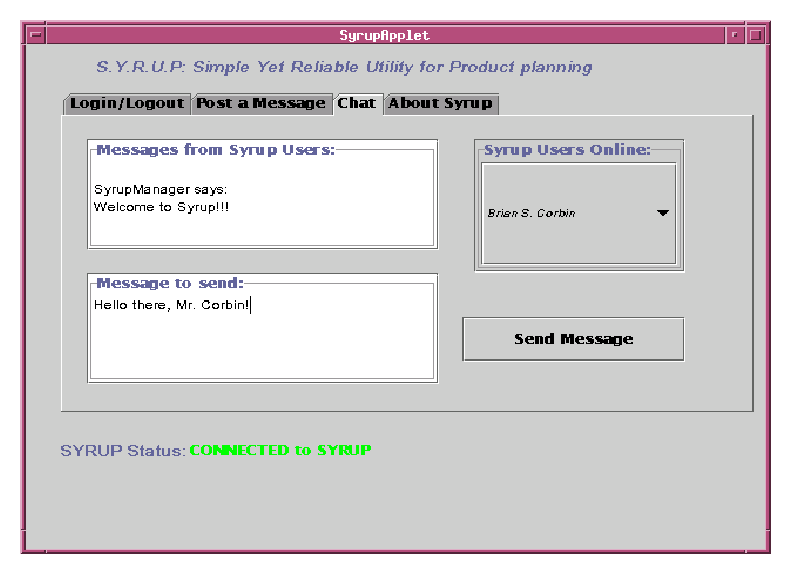
\psfig{file=Figures/syrup_screen_shot.eps}
\leavevmode
\caption{\em{Screen Capture of a SYRUP client application implemented in JAVA}.}
\figline
         \label{SyrupScreenShot}
\end{center}
\end{figure}

\section*{\underline{Performance}}
\addcontentsline{toc}{section}{Performance}

One factor that can influence the selection of an implementation language for a 
CORBA object is performance.  Clearly, we would like for our CORBA objects to
respond as quickly as possible to client application requests.  While this response
time is greatly influenced by the ORB in use, the implementation language can 
play a factor in how quickly operations are executed.  In this section, 
we conduct a performance experiment to compare two different implementations 
of the SyrupManager object using the same Object Request Broker, ORBit.   

\subsection*{The Experiment}
\addcontentsline{toc}{subsection}{The Experiment}

In order to determine if CORBA objects implemented in ML can provide 
satisfactory performance,  the SyrupManager object was re-implemented in C.
A Java application was written to repeatedly invoke the Login and Logout 
operations of the SyrupManager object and report the average time it took 
to execute the each operation.  The Java application was executed on a 
Sparc Ultra 5 with 128 Megabytes of physical memory running Solaris 7 using the 
Java Runtime Environment 1.3.  Both implementations of the SyrupManager 
object were executed on a PC with a Pentium 166 MHz processor and 64 Megabytes 
of physical memory running RedHat Linux 6.2.  ORBit version 0.5.6 was used 
as the Object Request Broker for both implementations. The C version of the 
SyrupManager object was compiled with gcc version 2.91.66. (No optimizations 
were used.)  


\subsection*{Experiment Results}
\addcontentsline{toc}{subsection}{Experiment Results}

The results from the experiment are shown in figure \ref{PerformanceResults}.
As the figure indicates, the ML implementation offers performance parallel to the 
C implementation.  As the number of invocations increases, it seems as though the 
C implementation performs slightly better on average.  This performance difference 
could be attributed to ML garbage collection.  
\begin{figure}
\begin{center}
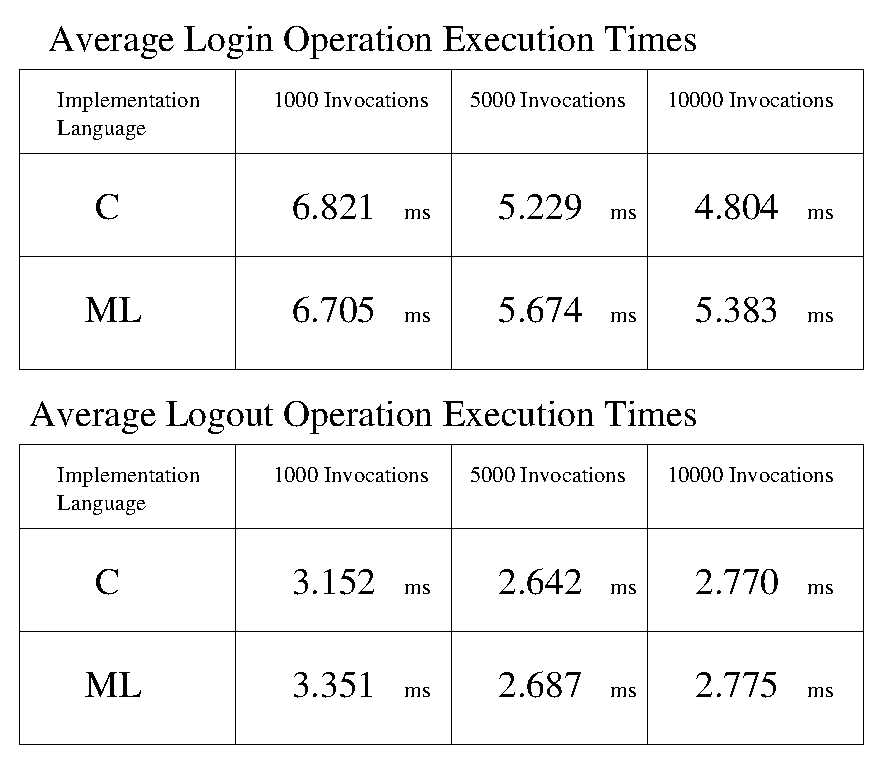
\psfig{file=Figures/PerformanceResults.eps}
\leavevmode
\caption{\em{Timings for Login and Logout operation invocations on two different implementations of the SyrupManager object}.}
\figline
         \label{PerformanceResults}
\end{center}
\end{figure}


